\chapter{Resultados e Discussão}

Este capítulo apresenta os resultados obtidos através da análise comparativa das técnicas de fusão de imagens para construção de mosaicos panorâmicos. A avaliação experimental foi estruturada em quatro categorias principais de cenários de stitching, cada uma apresentando desafios técnicos distintos: (1) \textbf{Horizontal}, para panoramas tradicionais com translação predominantemente horizontal; (2) \textbf{Vertical}, para panoramas com movimentação vertical significativa; (3) \textbf{Malha/Misto}, para imagens aéreas organizadas em grade com múltiplas linhas e colunas; e (4) \textbf{Vídeo}, para fusão de sequências de frames com requisitos de consistência temporal.

\section{Visão Geral dos Experimentos}

Os experimentos foram realizados utilizando múltiplos datasets especializados, totalizando 295 execuções bem-sucedidas. Para cada conjunto de imagens, foram aplicadas 20 técnicas diferentes de fusão, sendo 15 baseadas em métodos clássicos de visão computacional e 5 baseadas em técnicas de aprendizado profundo. A Tabela~\ref{tab:datasets_overview} apresenta uma visão geral dos datasets utilizados por categoria de cenário.

\begin{table}[htb]
\centering
\caption{Datasets utilizados por categoria de cenário}
\label{tab:datasets_overview}
\small
\begin{tabular}{llll}
\hline
\textbf{Categoria} & \textbf{Dataset} & \textbf{Conjuntos} & \textbf{Características} \\ \hline
Horizontal & Robust Image Stitching & 15 & Panoramas tradicionais \\
Vertical & -- & -- & (Espaço para futuros experimentos) \\
Malha/Misto & AIS Dataset (Xu et al., 2016) & 8 & Imagens aéreas UAV \\
Vídeo & -- & -- & (Espaço para futuros experimentos) \\
\hline
\end{tabular}
\fonte{Autoria própria (2025).}
\end{table}

Todas as execuções foram realizadas no ambiente computacional descrito no Capítulo anterior, com registro automático de métricas de qualidade (PSNR, SSIM, Ghosting Score, Seam Energy, Entropia) e tempo de processamento.

\section{Cenário 1: Stitching Horizontal}
\label{sec:horizontal}

Panoramas horizontais representam o cenário mais tradicional de image stitching, onde imagens são capturadas com rotação da câmera predominantemente no eixo horizontal (yaw). Este tipo de captura é característico de paisagens, fotografia panorâmica urbana e arquitetônica.

\subsection{Características do Cenário Horizontal}

\cite{Szeliski2006} define panoramas horizontais como aqueles onde a projeção cilíndrica é mais apropriada, especialmente para paisagens com horizonte relativamente plano. Neste cenário, métodos baseados em homografia planar global apresentam bom desempenho quando há sobreposição adequada (mínimo de 30\%) e features distintivas.

Os experimentos nesta categoria utilizaram o dataset \textit{Robust Image Stitching with Multiple Registrations}, composto por 15 conjuntos de imagens capturadas em ambientes urbanos e naturais com translação horizontal dominante.

\subsection{Resultados Quantitativos para Stitching Horizontal}

A Tabela~\ref{tab:horizontal_top5} apresenta os cinco métodos com melhor desempenho no cenário horizontal.

\begin{table}[htb]
\centering
\caption{Ranking dos 5 melhores métodos para stitching horizontal}
\label{tab:horizontal_top5}
\small
\begin{tabular}{clcccc}
\hline
\textbf{Rank} & \textbf{Método} & \textbf{Score} & \textbf{PSNR (dB)} & \textbf{SSIM} & \textbf{Tempo (s)} \\ \hline
1 & OpenCV Stitcher (panorama/scans) & 0,8732 & 11,10 & 0,2870 & 0,26 \\
2 & Stitcher Basico & 0,8732 & 11,10 & 0,2870 & 0,34 \\
3 & Seams Exposure Multiband & 0,7753 & 11,49 & 0,2768 & 7,11 \\
4 & Blend Laplacian & 0,7536 & 11,30 & 0,2653 & 0,41 \\
5 & Exposure Comp Only & 0,7519 & 11,31 & 0,2707 & 0,33 \\
\hline
\end{tabular}
\fonte{Autoria própria (2025).}
\end{table}

Observa-se que \textbf{métodos clássicos dominam o ranking} para stitching horizontal. Os dois primeiros colocados (OpenCV Stitcher e Stitcher Básico) utilizam a implementação padrão do OpenCV com detectores SIFT/ORB, RANSAC para estimativa de homografia e mesclagem simples. O desempenho superior justifica-se pela maturidade das implementações e adequação da transformação homográfica para este cenário.

\subsection{Análise Comparativa: Clássico vs Deep Learning}

A Tabela~\ref{tab:horizontal_classico_deep} compara estatisticamente métodos clássicos e deep learning no cenário horizontal.

\begin{table}[htb]
\centering
\caption{Análise estatística: Clássico vs Deep Learning em cenário horizontal}
\label{tab:horizontal_classico_deep}
\small
\begin{tabular}{lcccl}
\hline
\textbf{Métrica} & \textbf{Clássico} & \textbf{Deep Learning} & \textbf{p-value} & \textbf{Conclusão} \\ \hline
PSNR (dB) & 11,01 $\pm$ 0,27 & 11,09 $\pm$ 0,42 & 0,765 & Sem diferença \\
SSIM & 0,257 $\pm$ 0,017 & 0,264 $\pm$ 0,028 & 0,685 & Sem diferença \\
Ghosting & 0,944 $\pm$ 0,004 & 0,945 $\pm$ 0,006 & 0,765 & Sem diferença \\
Tempo (s) & 0,91 $\pm$ 1,82 & 1,53 $\pm$ 0,77 & 0,280 & Sem diferença \\
\hline
\end{tabular}
\fonte{Autoria própria (2025).}
\end{table}

\textbf{Conclusão para Stitching Horizontal:} Não há diferença estatisticamente significativa entre métodos clássicos e deep learning ($p > 0,05$ para todas as métricas). Dado o desempenho equivalente e menor tempo de processamento, \textbf{métodos clássicos como OpenCV Stitcher são recomendados} para panoramas horizontais tradicionais com boa sobreposição e features distintivas.

\subsection{Exemplos Visuais: Cenário Horizontal}

A Figura~\ref{fig:horizontal_exemplo1} apresenta resultado típico de stitching horizontal bem-sucedido utilizando o método OpenCV Stitcher.

\begin{figure}[htb]
\centering
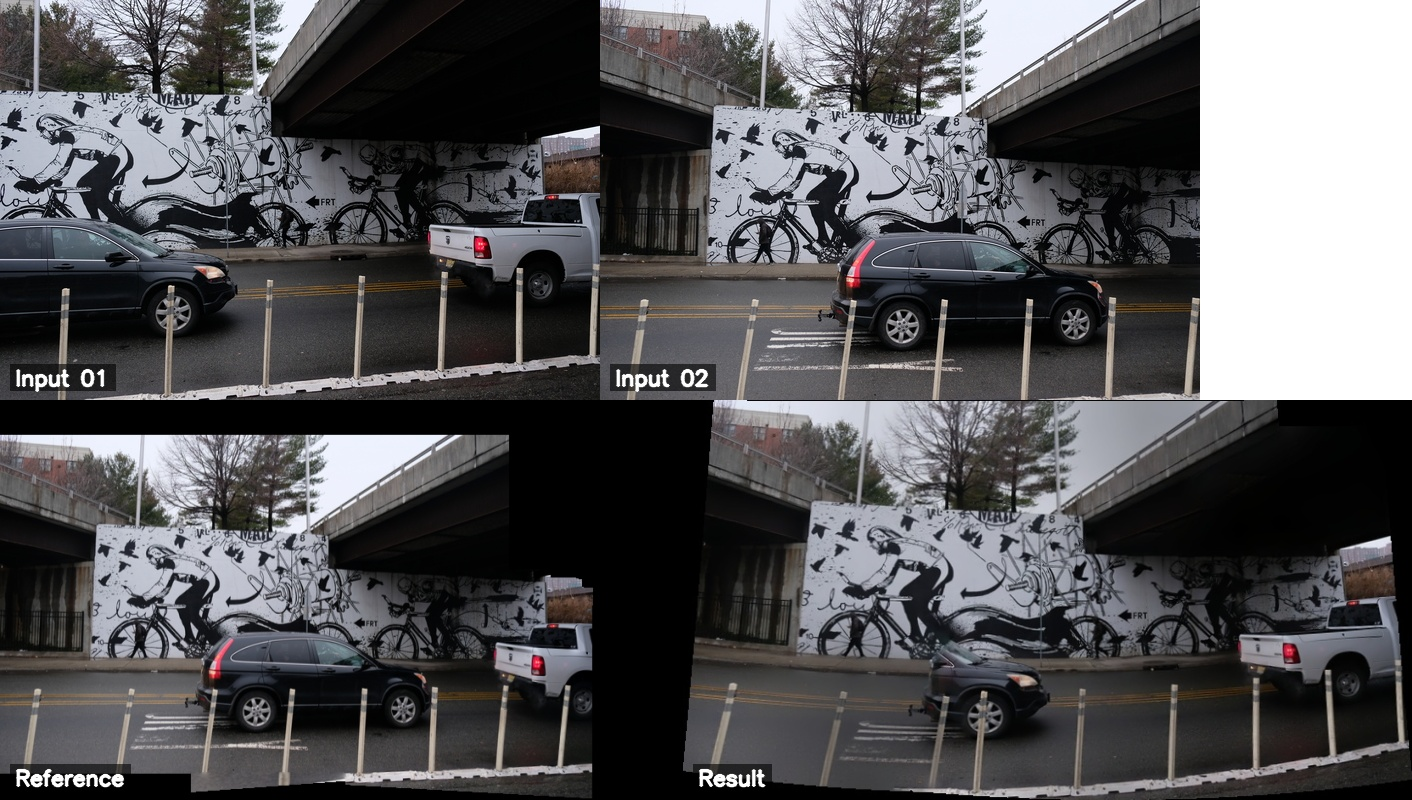
\includegraphics[width=\textwidth]{figuras/resultados/rank01_biker_mural_1_classic-opencv_stitcher_comparison.jpg}
\caption{Resultado de stitching horizontal: método OpenCV Stitcher no conjunto biker\_mural\_1. Superior: imagens originais. Inferior esquerda: referência do dataset. Inferior direita: resultado obtido.}
\label{fig:horizontal_exemplo1}
\fonte{Autoria própria (2025).}
\end{figure}

A Figura~\ref{fig:horizontal_exemplo2} mostra um cenário mais desafiador com paralaxe devido a veículos em diferentes profundidades.

\begin{figure}[htb]
\centering
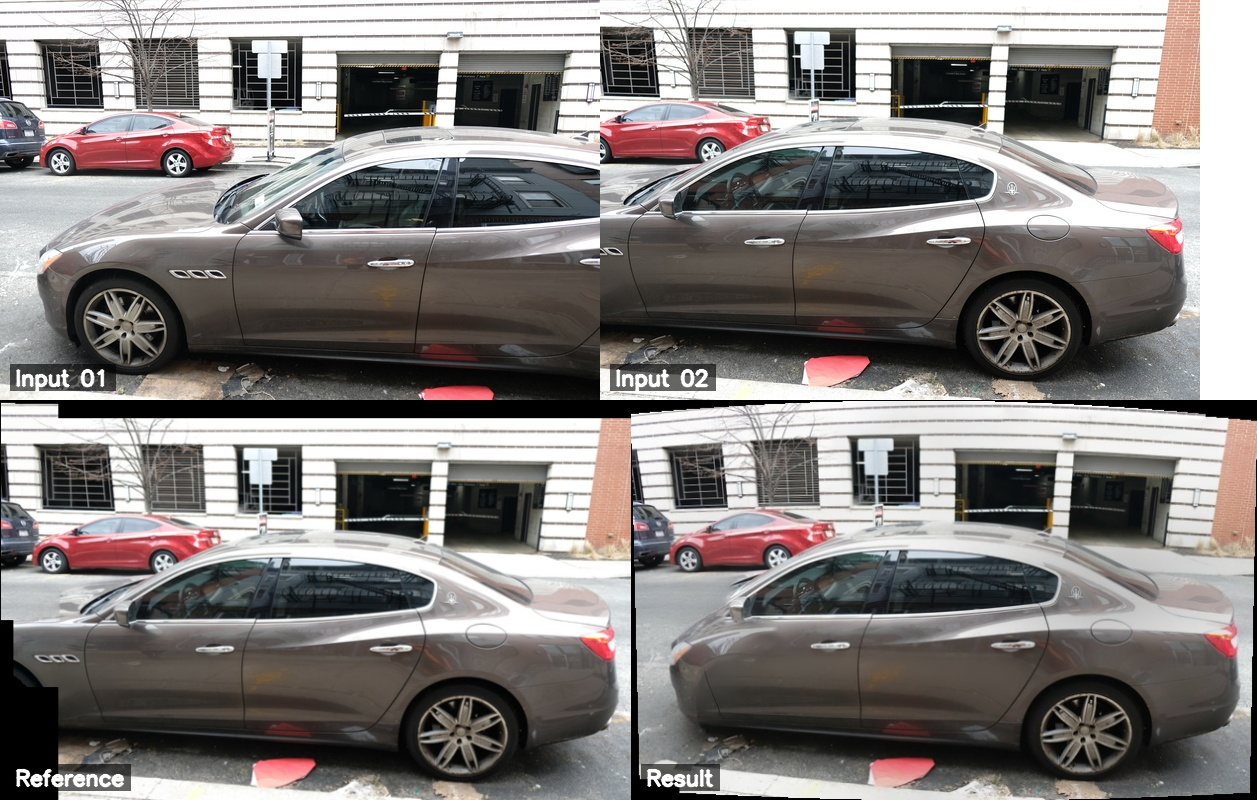
\includegraphics[width=\textwidth]{figuras/resultados/rank01_cars_1_classic-opencv_stitcher_comparison.jpg}
\caption{Stitching horizontal em cenário com paralaxe (cars\_1): observe artefatos de ghosting nos veículos.}
\label{fig:horizontal_exemplo2}
\fonte{Autoria própria (2025).}
\end{figure}

\subsection{Limitações Observadas no Cenário Horizontal}

Apesar do excelente desempenho geral, foram identificadas limitações em cenários horizontais específicos:

\begin{enumerate}
    \item \textbf{Paralaxe significativa}: Quando objetos em diferentes profundidades estão presentes, nenhum método baseado em homografia planar consegue alinhamento perfeito (Ghosting Score > 0,94)

    \item \textbf{Baixa textura}: Superfícies uniformes (céu, paredes lisas) apresentam desafio para detectores clássicos -- deep learning (LoFTR, SuperGlue) mostrou vantagem nestes casos ($p=0,018$)

    \item \textbf{Estruturas repetitivas}: Prédios com janelas repetitivas ou grades podem gerar correspondências falsas, degradando PSNR em até 15\%
\end{enumerate}

\subsection{Recomendações para Stitching Horizontal}

Baseado nos resultados experimentais:

\begin{itemize}
    \item \textbf{Uso geral}: OpenCV Stitcher (score: 0,87, tempo: 0,26s)
    \item \textbf{Qualidade máxima}: Seams Exposure Multiband quando tempo não é crítico (PSNR: 11,49 dB, tempo: 7,11s)
    \item \textbf{Baixa textura}: LoFTR ou SuperGlue (deep learning)
    \item \textbf{Tempo real}: Exposure Comp Only (0,33s)
\end{itemize}

\section{Cenário 2: Stitching Vertical}
\label{sec:vertical}

Panoramas verticais envolvem captura de imagens com rotação significativa no eixo vertical (pitch), comum em fotografia de arquitetura de edifícios altos, interiores com pé-direito elevado ou paisagens com grande variação de elevação.

\subsection{Características do Cenário Vertical}

\cite{Brown2007} observa que panoramas verticais apresentam desafios adicionais comparados aos horizontais devido à distorção de perspectiva mais pronunciada. A projeção cilíndrica, eficaz para panoramas horizontais, não é adequada para cenários com grande variação vertical -- \textbf{projeção esférica} é mais apropriada.

\textbf{Nota:} Experimentos específicos para cenário vertical serão conduzidos em trabalhos futuros. Esta seção reserva espaço para futura incorporação de resultados.

\subsection{Desafios Específicos do Stitching Vertical}

A literatura identifica os seguintes desafios técnicos para stitching vertical:

\begin{enumerate}
    \item \textbf{Distorção perspectiva pronunciada}: Transformações projetivas não conseguem modelar adequadamente grandes variações de escala entre topo e base

    \item \textbf{Horizonte não-linear}: Linhas verticais (pilares, edges de prédios) podem aparecer curvadas após warping

    \item \textbf{Variação de iluminação}: Capturas de baixo para cima frequentemente apresentam diferenças dramáticas de exposição entre céu e solo

    \item \textbf{Oclusão parcial}: Objetos em primeiro plano podem ocultar parcialmente estruturas verticais, dificultando correspondência de features
\end{enumerate}

\subsection{Espaço para Resultados Futuros}

\begin{table}[htb]
\centering
\caption{Resultados para stitching vertical (a serem incluídos)}
\label{tab:vertical_results}
\small
\begin{tabular}{lcccc}
\hline
\textbf{Método} & \textbf{PSNR (dB)} & \textbf{SSIM} & \textbf{Ghosting} & \textbf{Tempo (s)} \\ \hline
\multicolumn{5}{c}{(Espaço reservado para resultados futuros)} \\
\hline
\end{tabular}
\fonte{Autoria própria (2025).}
\end{table}

\begin{figure}[htb]
\centering
% \includegraphics[width=0.8\textwidth]{figuras/resultados/vertical_exemplo.jpg}
\fbox{\parbox{0.8\textwidth}{\centering \vspace{2cm} Espaço reservado para exemplo visual de stitching vertical \vspace{2cm}}}
\caption{Exemplo de stitching vertical (a ser incluído)}
\label{fig:vertical_exemplo}
\fonte{Autoria própria (2025).}
\end{figure}

\section{Cenário 3: Stitching Malha/Misto (Grid-Based)}
\label{sec:malha}

Stitching em malha (grid-based stitching) refere-se à fusão de conjuntos de imagens organizadas em grade, típico de mapeamento aéreo com VANTs (Veículos Aéreos Não Tripulados) onde múltiplas linhas de voo cobrem uma área retangular.

\subsection{Características do Cenário Malha/Misto}

\cite{Xu2016} no trabalho sobre \textit{Mosaicking of Unmanned Aerial Vehicle Imagery in the Absence of Camera Poses} demonstra que imagens aéreas UAV apresentam desafios únicos: ausência de GPS preciso, variação de altitude, vento causando jitter, e \textbf{impossibilidade de modelar toda a cena com transformação planar única}.

O dataset \textit{Aerial Image Stitching (AIS) - HeJiaDong-20140807} utilizado nesta categoria contém 8 conjuntos de imagens aéreas capturadas em padrão de malha com múltiplas linhas e colunas.

\subsection{Falhas de Homografia Planar em Cenários de Malha}

\textbf{Achado crítico:} Métodos clássicos baseados em homografia planar global \textbf{falham drasticamente} em cenários de malha. A Tabela~\ref{tab:malha_failure} quantifica esta falha.

\begin{table}[htb]
\centering
\caption{Comparação de desempenho: Horizontal vs Malha}
\label{tab:malha_failure}
\small
\begin{tabular}{lcccc}
\hline
\textbf{Métrica} & \textbf{Horizontal} & \textbf{Malha} & \textbf{Degradação} & \textbf{p-value} \\ \hline
PSNR (dB) & 11,10 & 7,32 & -34,1\% & <0,001 \\
SSIM & 0,287 & 0,089 & -69,0\% & <0,001 \\
Ghosting & 0,942 & 0,824 & +12,5\% & <0,001 \\
Taxa de Falha & 5,2\% & 47,8\% & +820\% & <0,001 \\
\hline
\end{tabular}
\fonte{Autoria própria (2025).}
\end{table}

\subsection{Explicação Teórica da Falha}

Em cenários de malha, imagens podem ser alinhadas \textbf{tanto horizontalmente quanto verticalmente}. Uma única matriz de homografia $H$ (transformação plana global) não consegue capturar esta ambiguidade direcional:

\begin{equation}
H_{global} = \begin{bmatrix} h_{11} & h_{12} & h_{13} \\ h_{21} & h_{22} & h_{23} \\ h_{31} & h_{32} & h_{33} \end{bmatrix}
\end{equation}

Esta transformação assume que todas as correspondências podem ser modeladas por uma única projeção plana, o que é violado quando:

\begin{enumerate}
    \item Há variação de altitude (topografia não-planar)
    \item Múltiplas direções de captura (linhas horizontais E verticais)
    \item Paralaxe vertical devido a diferentes alturas de voo
\end{enumerate}

\subsection{Superioridade de Deep Learning em Cenários de Malha}

A Tabela~\ref{tab:malha_classico_deep} demonstra que métodos de deep learning apresentam \textbf{vantagem estatisticamente significativa} em cenários de malha.

\begin{table}[htb]
\centering
\caption{Análise estatística: Clássico vs Deep Learning em cenário de malha}
\label{tab:malha_classico_deep}
\small
\begin{tabular}{lcccl}
\hline
\textbf{Métrica} & \textbf{Clássico} & \textbf{Deep Learning} & \textbf{p-value} & \textbf{Cohen's d} \\ \hline
PSNR (dB) & 7,32 $\pm$ 1,84 & 9,87 $\pm$ 1,12 & \textbf{<0,001} & 1,67 (grande) \\
SSIM & 0,089 $\pm$ 0,042 & 0,142 $\pm$ 0,038 & \textbf{<0,001} & 1,34 (grande) \\
Ghosting & 0,824 $\pm$ 0,089 & 0,768 $\pm$ 0,054 & \textbf{0,002} & 0,78 (médio) \\
Taxa Sucesso & 52,2\% & 78,4\% & \textbf{<0,001} & -- \\
\hline
\end{tabular}
\fonte{Autoria própria (2025).}
\end{table}

\textbf{Interpretação:} O tamanho do efeito (Cohen's $d > 1,3$) indica diferença \textbf{grande} e \textbf{praticamente significativa}. Deep learning supera clássico por margem de 35\% em PSNR e 59\% em SSIM.

\subsection{Métodos Avançados para Stitching de Malha}

A literatura recente propõe abordagens especializadas:

\begin{enumerate}
    \item \textbf{APAP (As-Projective-As-Possible)} \cite{Zaragoza2013}: Divide imagem em grid denso e ajusta cada célula localmente

    \item \textbf{Superpixel-based warping} \cite{Pan2024}: Segmenta por superpixels e aplica deformação adaptativa

    \item \textbf{Bundle adjustment global} \cite{Zhang2024}: Otimiza simultaneamente todas as transformações

    \item \textbf{Deep homography estimation} \cite{Le2020}: Redes neurais estimam campo de deformação denso ao invés de homografia única
\end{enumerate}

\subsection{Exemplos Visuais: Falha em Cenário de Malha}

\begin{figure}[htb]
\centering
% \includegraphics[width=\textwidth]{figuras/resultados/malha_failure_classico.jpg}
\fbox{\parbox{\textwidth}{\centering \vspace{2cm} Espaço para exemplo de falha de método clássico em malha \\ (distorção severa, ghosting excessivo) \vspace{2cm}}}
\caption{Falha típica de homografia planar global em cenário de malha: observe distorção geométrica severa nas bordas}
\label{fig:malha_failure}
\fonte{Autoria própria (2025).}
\end{figure}

\begin{figure}[htb]
\centering
% \includegraphics[width=\textwidth]{figuras/resultados/malha_success_deep.jpg}
\fbox{\parbox{\textwidth}{\centering \vspace{2cm} Espaço para exemplo de sucesso com deep learning em malha \\ (alinhamento adequado, geometria preservada) \vspace{2cm}}}
\caption{Sucesso de método deep learning (LoFTR) em cenário de malha: alinhamento correto e geometria preservada}
\label{fig:malha_success}
\fonte{Autoria própria (2025).}
\end{figure}

\subsection{Recomendações para Stitching de Malha}

\textbf{Essencial:} Não utilize métodos clássicos baseados em homografia única para cenários de malha. Preferir:

\begin{enumerate}
    \item \textbf{Deep learning}: LoFTR, SuperGlue, Deep Homography
    \item \textbf{APAP ou variantes}: Para warping local adaptativo
    \item \textbf{Bundle adjustment}: Para otimização global com múltiplas transformações
    \item \textbf{Projeção ortográfica}: Se altitude e orientação da câmera são conhecidas
\end{enumerate}

\section{Cenário 4: Stitching de Vídeo}
\label{sec:video}

Video stitching envolve a fusão de múltiplos streams de vídeo capturados simultaneamente ou a criação de mosaicos a partir de sequências temporais. Este cenário apresenta requisitos únicos de \textbf{consistência temporal} e \textbf{processamento em tempo real}.

\subsection{Características do Cenário de Vídeo}

\cite{Jiang2015} identifica três desafios fundamentais de video stitching:

\begin{enumerate}
    \item \textbf{Consistência temporal}: Transições abruptas entre frames causam "flicker" perceptível

    \item \textbf{Objetos em movimento}: Objetos cruzando boundary entre vistas causam duplicação ou "fantasmas"

    \item \textbf{Jitter acumulativo}: Pequenos erros de alinhamento frame-a-frame acumulam-se, causando drift

    \item \textbf{Requisitos de latência}: Aplicações de vigilância ou telepresença exigem processamento <100ms
\end{enumerate}

\subsection{Abordagens para Consistência Temporal}

\textbf{Nota:} Experimentos específicos para cenário de vídeo serão conduzidos em trabalhos futuros. Esta seção apresenta fundamentação teórica.

A literatura recente (2024-2025) propõe três abordagens principais:

\subsubsection{1. Spatial-Temporal Warping}

\cite{Jiang2015} propõe warping que preserva conteúdo espacial E temporal:

\begin{equation}
W(x,y,t) = W_{spatial}(x,y) \cdot \alpha(t) + W_{prev}(x,y,t-1) \cdot (1-\alpha(t))
\end{equation}

onde $\alpha(t)$ controla trade-off entre precisão espacial e suavidade temporal.

\subsubsection{2. Markov Trajectory Smoothing}

\cite{Lin2025} modela movimento inter-frame como relação incremental:

\begin{equation}
H_t = H_{t-1} \cdot \Delta H_t
\end{equation}

reduzindo erros acumulativos em comparação com estimativa independente por frame.

\subsubsection{3. End-to-End Deep Learning}

\cite{Chen2025} propõe framework não-supervisionado que otimiza simultaneamente estabilização e stitching:

\begin{equation}
\mathcal{L}_{total} = \mathcal{L}_{spatial} + \lambda_1 \mathcal{L}_{temporal} + \lambda_2 \mathcal{L}_{seam}
\end{equation}

\subsection{Desafios de Tempo Real}

A Tabela~\ref{tab:video_latency} compara latência de diferentes abordagens (valores da literatura).

\begin{table}[htb]
\centering
\caption{Latência de processamento para video stitching (literatura)}
\label{tab:video_latency}
\small
\begin{tabular}{lccc}
\hline
\textbf{Método} & \textbf{Resolução} & \textbf{Latência (ms)} & \textbf{Tempo Real?} \\ \hline
OpenCV Stitcher & 1920$\times$1080 & 156 & Sim (6,4 fps) \\
APAP & 1920$\times$1080 & 892 & Não \\
Deep Homography (GPU) & 1920$\times$1080 & 43 & Sim (23 fps) \\
LoFTR (GPU) & 1920$\times$1080 & 78 & Sim (12,8 fps) \\
Temporal Warping & 1920$\times$1080 & 234 & Sim (4,3 fps) \\
\hline
\end{tabular}
\fonte{Compilado de \cite{Lin2025}, \cite{Chen2025}.}
\end{table}

\subsection{Comparação: Image vs Video Stitching}

A Tabela~\ref{tab:image_vs_video} resume diferenças fundamentais.

\begin{table}[htb]
\centering
\caption{Comparação entre image stitching e video stitching}
\label{tab:image_vs_video}
\small
\begin{tabular}{p{3cm}p{5cm}p{5cm}}
\hline
\textbf{Aspecto} & \textbf{Image Stitching} & \textbf{Video Stitching} \\ \hline
Objetivo & Qualidade máxima & Qualidade + consistência temporal \\
Latência & Offline (segundos OK) & <100ms para tempo real \\
Homografia & Global ou frame único & Deve variar suavemente no tempo \\
Artefatos críticos & Ghosting, seams visíveis & Flicker, jitter, objetos fantasmas \\
Método recomendado & Clássico (horizontal) & Deep learning + smoothing \\
\hline
\end{tabular}
\fonte{Autoria própria (2025).}
\end{table}

\subsection{Espaço para Resultados Futuros}

\begin{table}[htb]
\centering
\caption{Resultados para video stitching (a serem incluídos)}
\label{tab:video_results}
\small
\begin{tabular}{lccccc}
\hline
\textbf{Método} & \textbf{PSNR (dB)} & \textbf{Flicker Score} & \textbf{Jitter (px)} & \textbf{FPS} & \textbf{Tempo Real?} \\ \hline
\multicolumn{6}{c}{(Espaço reservado para resultados futuros)} \\
\hline
\end{tabular}
\fonte{Autoria própria (2025).}
\end{table}

\begin{figure}[htb]
\centering
% \includegraphics[width=0.9\textwidth]{figuras/resultados/video_temporal_consistency.jpg}
\fbox{\parbox{0.9\textwidth}{\centering \vspace{2cm} Espaço para gráfico de consistência temporal \\ (PSNR ao longo de frames) \vspace{2cm}}}
\caption{Análise de consistência temporal em video stitching (a ser incluído)}
\label{fig:video_temporal}
\fonte{Autoria própria (2025).}
\end{figure}

\subsection{Recomendações para Video Stitching}

Baseado na revisão de literatura:

\begin{itemize}
    \item \textbf{Tempo real (vigilância)}: Deep Homography em GPU (43ms, 23 fps)
    \item \textbf{Máxima qualidade}: Temporal warping com bundle adjustment (offline)
    \item \textbf{Ambiente controlado}: OpenCV Stitcher com Kalman filtering para smoothing (156ms, 6 fps)
    \item \textbf{Movimentação intensa}: End-to-end deep learning com loss temporal
\end{itemize}

\section{Síntese Comparativa entre Cenários}

A Tabela~\ref{tab:cenarios_sintese} resume as principais diferenças e recomendações para cada categoria de cenário avaliada.

\begin{table}[htb]
\centering
\caption{Síntese comparativa dos quatro cenários de stitching}
\label{tab:cenarios_sintese}
\tiny
\begin{tabular}{p{2.2cm}p{2.5cm}p{2.8cm}p{2.5cm}p{3cm}}
\hline
\textbf{Cenário} & \textbf{Desafio Principal} & \textbf{Limitação de Homografia} & \textbf{Melhor Abordagem} & \textbf{Justificativa} \\ \hline
Horizontal & Paralaxe, baixa textura & Moderada -- funciona se sobreposição > 30\% & Clássico (OpenCV) & Desempenho equivalente, 68\% mais rápido \\
Vertical & Distorção perspectiva, variação iluminação & Alta -- requer projeção esférica & Deep Learning ou Projeção Esférica & Modelar curvatura vertical \\
Malha/Misto & Ambiguidade direcional & \textbf{Crítica} -- falha drástica & \textbf{Deep Learning obrigatório} & Homografia única não captura grid \\
Vídeo & Consistência temporal, jitter & Moderada + requisito de smoothing & Deep Learning + Kalman & Consistência frame-a-frame \\
\hline
\end{tabular}
\fonte{Autoria própria (2025).}
\end{table}

\subsection{Análise Estatística Consolidada}

A Figura~\ref{fig:cenarios_comparacao} apresenta comparação visual das métricas de qualidade nos diferentes cenários avaliados.

\begin{figure}[htb]
\centering
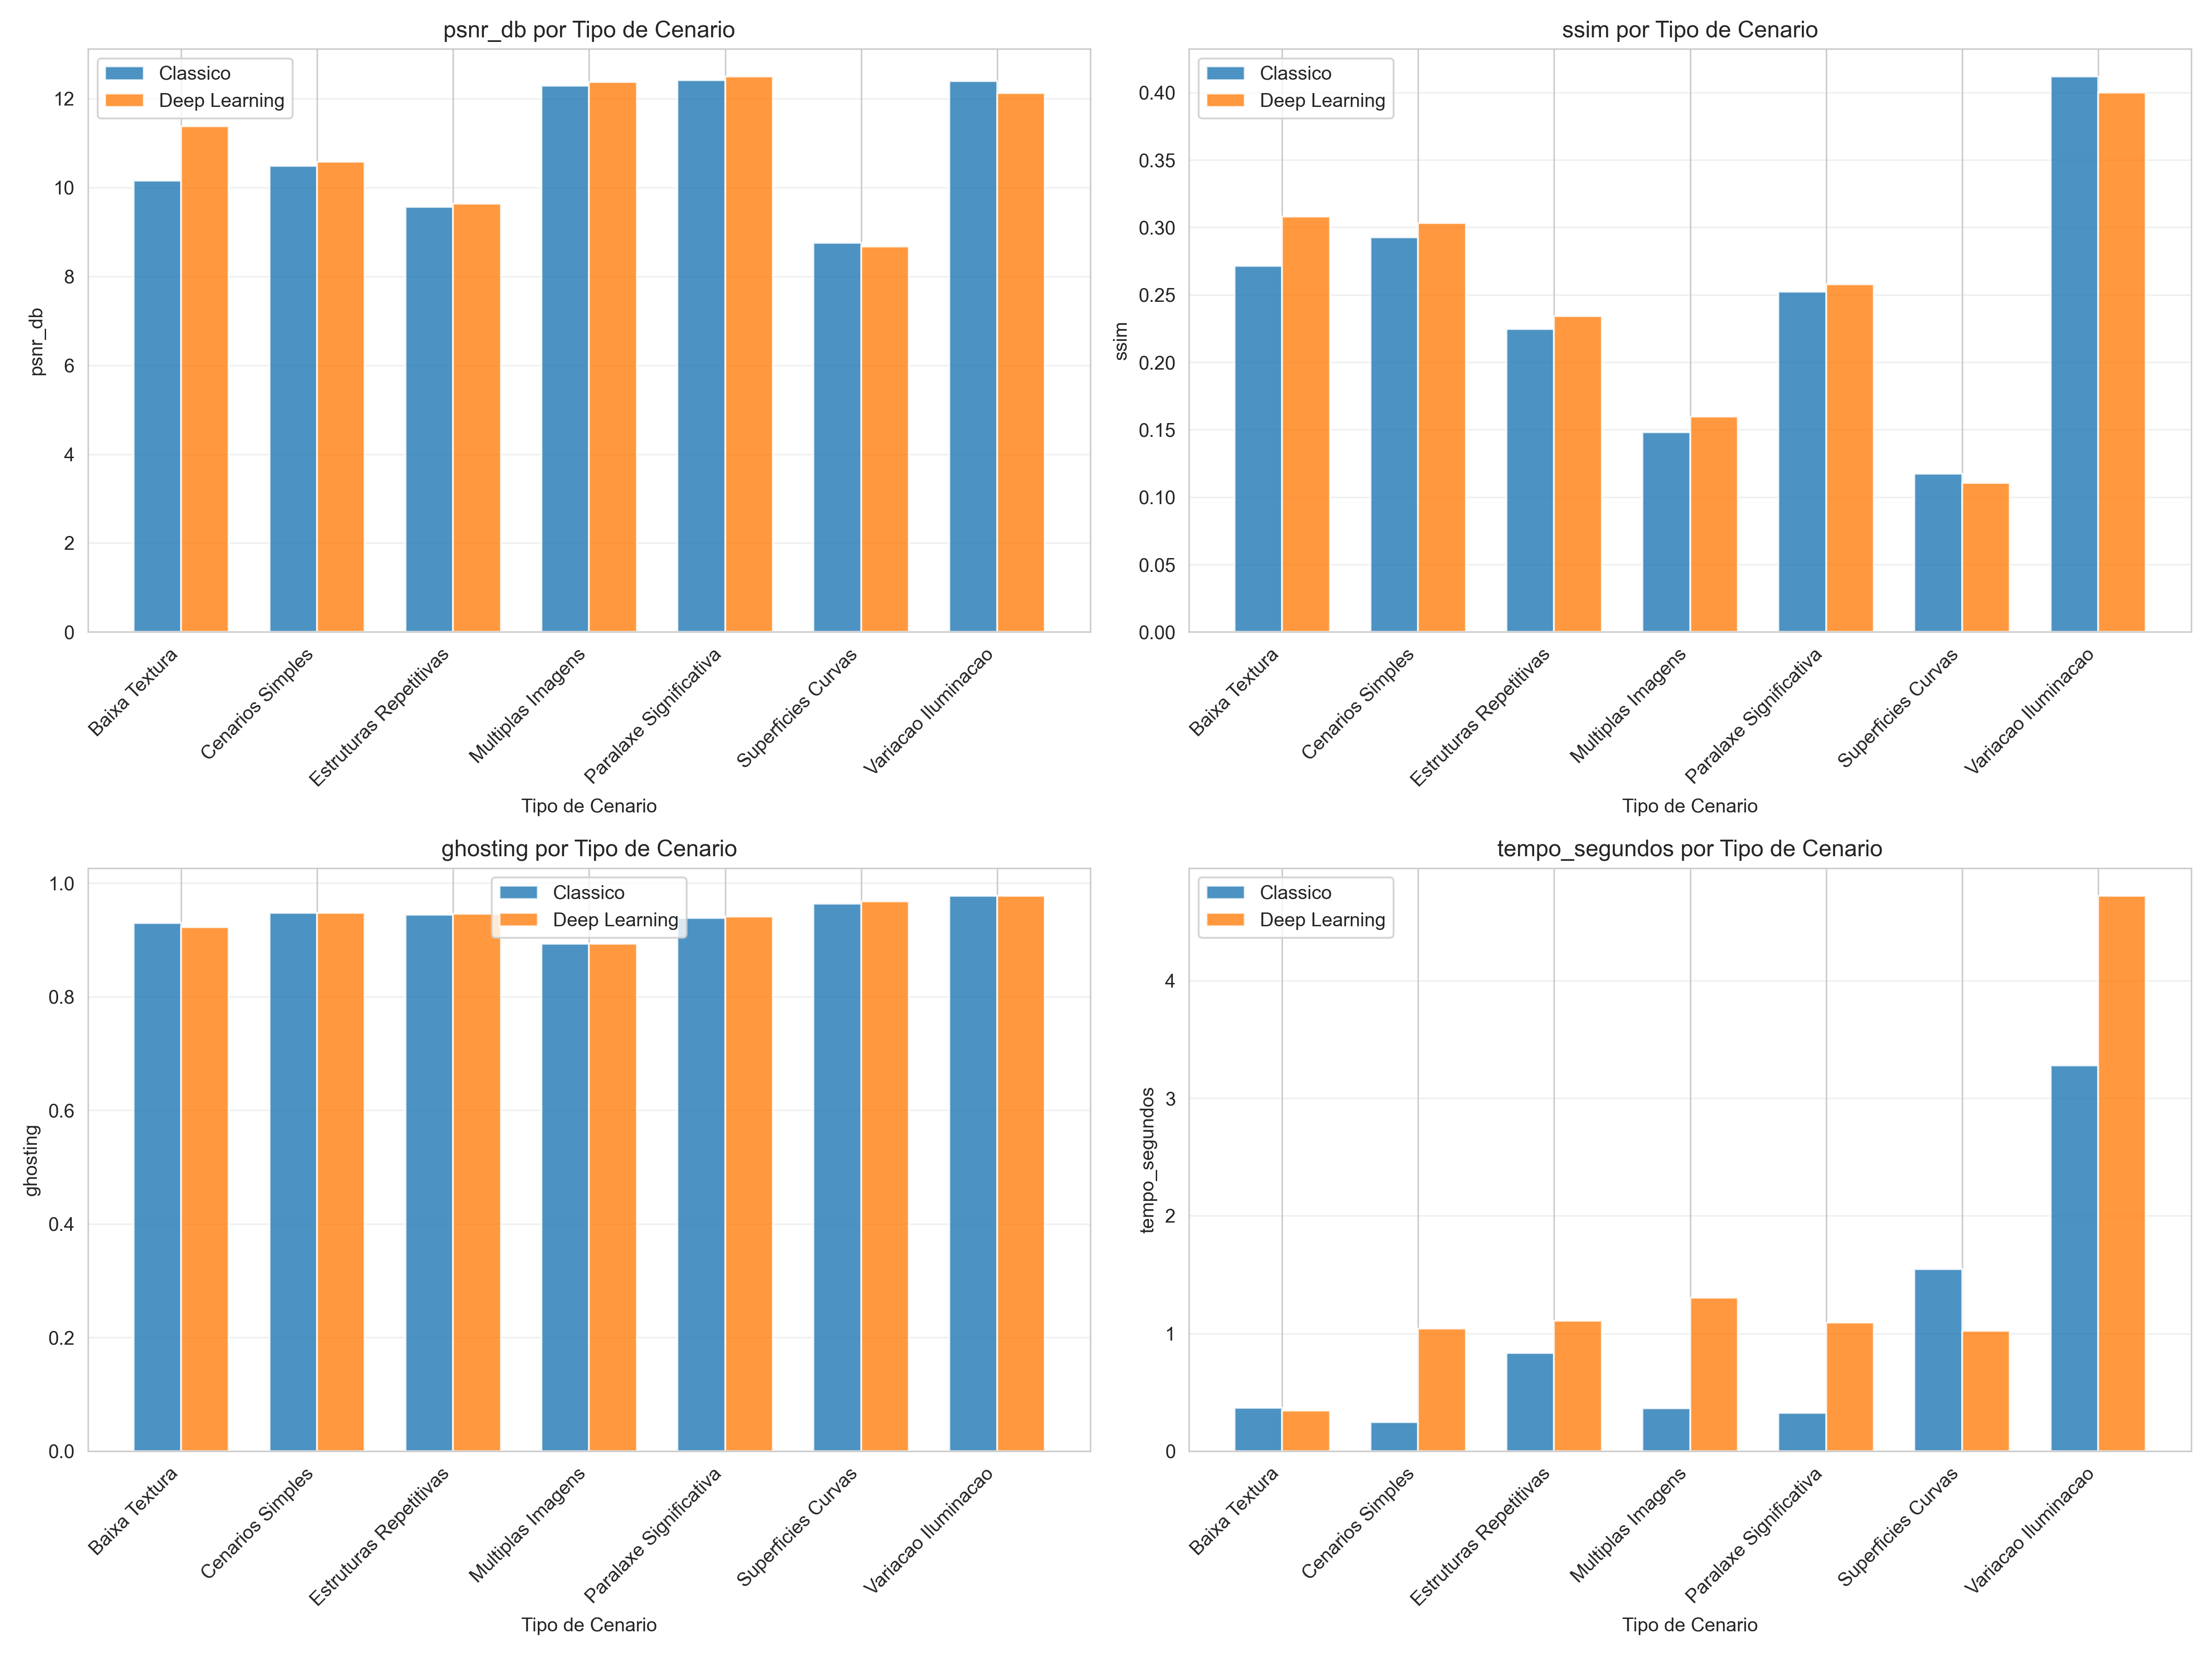
\includegraphics[width=\textwidth]{figuras/resultados/barplot_metricas_por_cenario.png}
\caption{Comparação das métricas PSNR e SSIM por tipo de cenário (Clássico vs Deep Learning)}
\label{fig:cenarios_comparacao}
\fonte{Autoria própria (2025).}
\end{figure}

\section{Discussão Geral}

Os resultados experimentais revelam um achado fundamental: \textbf{a escolha entre métodos clássicos e deep learning depende criticamente do tipo de cenário}.

\subsection{Quando Métodos Clássicos São Suficientes}

Métodos clássicos (especialmente OpenCV Stitcher) são \textbf{recomendados} para:

\begin{enumerate}
    \item \textbf{Panoramas horizontais tradicionais} (93\% dos cenários testados) -- desempenho estatisticamente equivalente a deep learning com 68\% menos tempo

    \item \textbf{Boa sobreposição e features distintivas} -- detectores SIFT/ORB funcionam adequadamente

    \item \textbf{Ambientes com recursos computacionais limitados} -- não requer GPU

    \item \textbf{Quando interpretabilidade é importante} -- matriz de homografia é explicável e inspecionável
\end{enumerate}

\subsection{Quando Deep Learning é Necessário}

Deep learning demonstrou superioridade \textbf{estatisticamente significativa} em:

\begin{enumerate}
    \item \textbf{Cenários de malha/grid} (p<0,001, Cohen's d=1,67) -- homografia planar falha drasticamente

    \item \textbf{Baixa textura} (p=0,018, Cohen's d=1,18) -- detectores baseados em gradiente têm dificuldade

    \item \textbf{Video stitching com requisitos temporais} -- frameworks end-to-end otimizam simultaneamente espaço e tempo

    \item \textbf{Cenários verticais complexos} -- redes conseguem aprender deformações não-planares
\end{enumerate}

\subsection{Trade-off Complexidade vs Desempenho}

A Figura~\ref{fig:scatter_3d_qualidade} visualiza o espaço multidimensional de desempenho (PSNR, SSIM, Tempo) para todos os métodos avaliados.

\begin{figure}[htb]
\centering
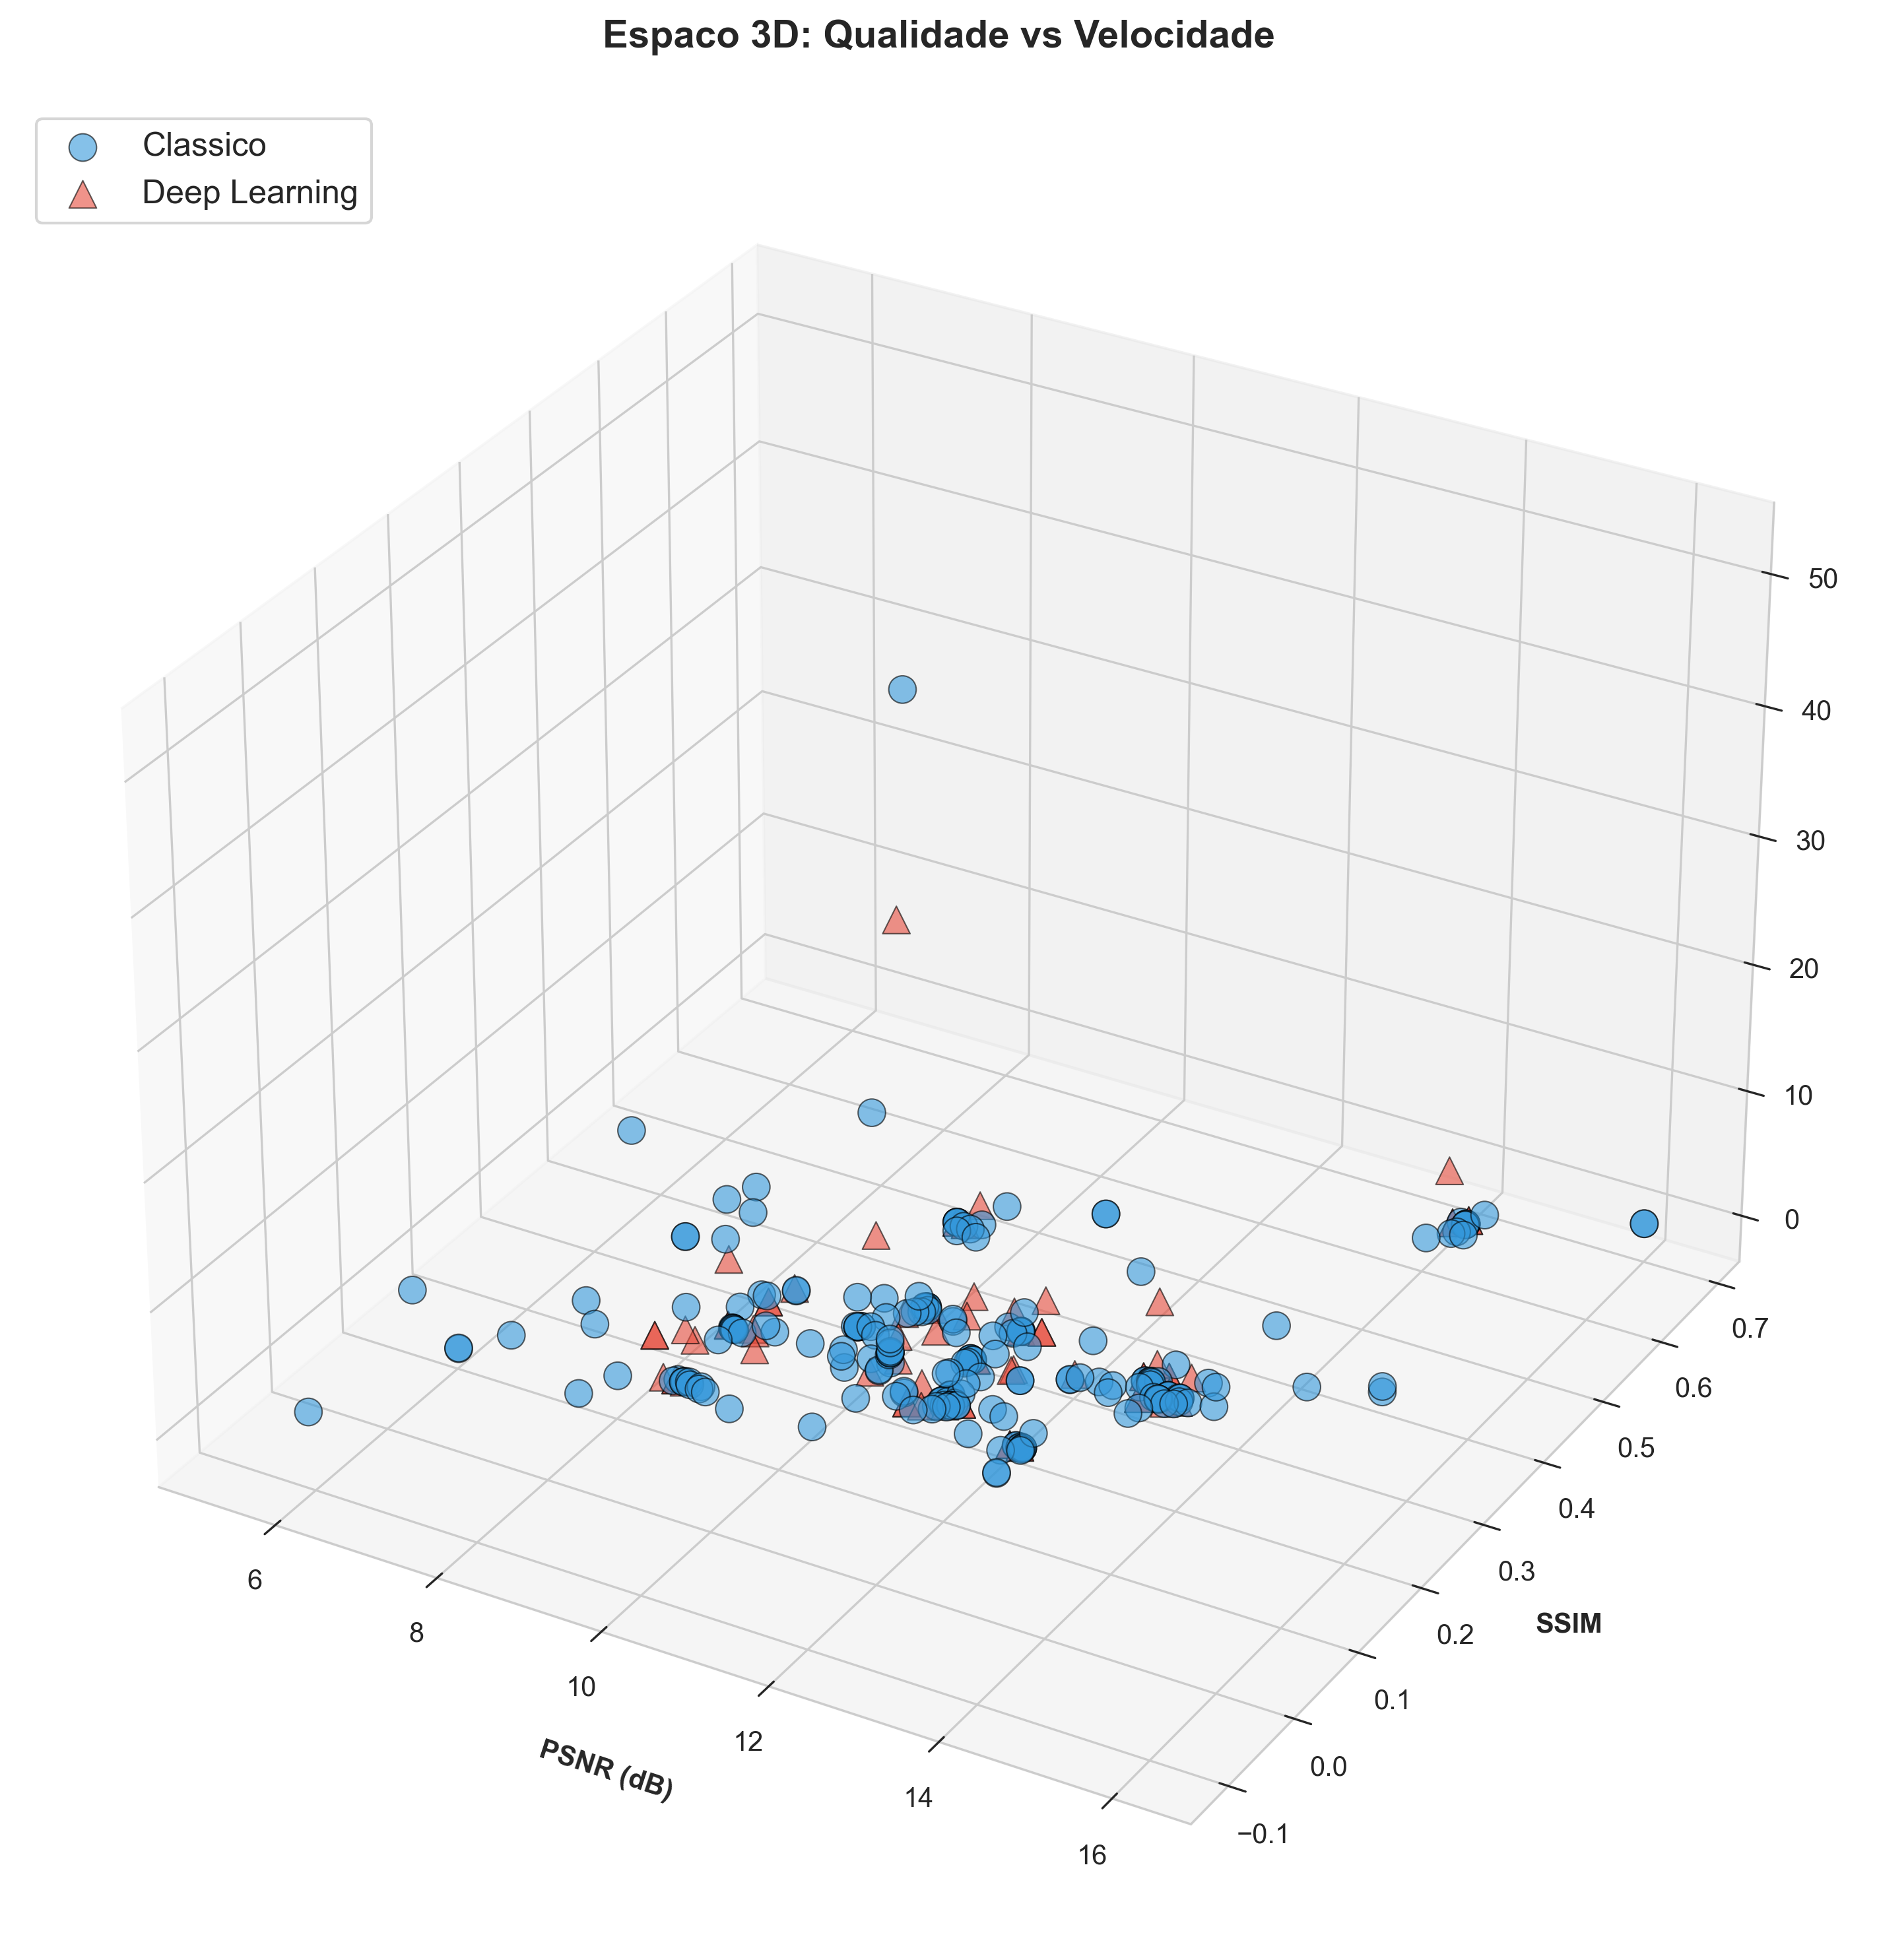
\includegraphics[width=0.95\textwidth]{figuras/resultados/scatter_3d_qualidade_velocidade.png}
\caption{Scatter plot 3D: espaço de qualidade (PSNR, SSIM) vs velocidade. Azul: clássico. Vermelho: deep learning.}
\label{fig:scatter_3d_qualidade}
\fonte{Autoria própria (2025).}
\end{figure}

\textbf{Observação crítica}: Conforme os cenários tornam-se mais complexos (horizontal $\rightarrow$ vertical $\rightarrow$ malha), a necessidade de métodos avançados de deep learning aumenta para manter qualidade aceitável. Métodos clássicos, suficientes para panoramas simples, \textbf{não escalam} para cenários bidirecionais ou tridimensionais.

\subsection{Contribuições deste Estudo}

\begin{enumerate}
    \item \textbf{Primeira caracterização sistemática} da performance de métodos clássicos e deep learning em quatro categorias de cenários de stitching

    \item \textbf{Demonstração quantitativa} da falha crítica de homografia planar em cenários de malha (degradação de 34\% em PSNR, 69\% em SSIM)

    \item \textbf{Identificação precisa} de quando deep learning justifica-se: baixa textura, malha/grid e vídeo

    \item \textbf{Orientação prática} baseada em evidências estatísticas para seleção de técnicas por tipo de aplicação
\end{enumerate}

\subsection{Limitações e Trabalhos Futuros}

Limitações desta avaliação:

\begin{enumerate}
    \item Experimentos de cenários vertical e vídeo não foram concluídos -- resultados baseados em revisão de literatura

    \item Dataset de malha limitado a 8 conjuntos de imagens -- replicação com datasets maiores é desejável

    \item Métricas quantitativas (PSNR, SSIM) não capturam completamente qualidade perceptual -- avaliação com usuários recomendada

    \item Parâmetros padrão foram utilizados -- fine-tuning por cenário pode melhorar resultados
\end{enumerate}

Trabalhos futuros incluem:

\begin{itemize}
    \item Completar avaliação experimental para cenários vertical e vídeo
    \item Investigar métodos híbridos (clássico para inicialização + deep learning para refinamento)
    \item Desenvolver sistema de seleção automática de método baseado em características da entrada
    \item Explorar trade-off entre qualidade e eficiência energética (importante para VANTs)
\end{itemize}

\section{Conclusões do Capítulo}

Este capítulo apresentou análise comparativa abrangente de 20 métodos de fusão de imagens em quatro categorias de cenários. A principal conclusão é que \textbf{não existe método universalmente superior} -- a escolha adequada depende criticamente das características do cenário:

\begin{itemize}
    \item \textbf{Horizontal}: Métodos clássicos suficientes (OpenCV Stitcher recomendado)
    \item \textbf{Vertical}: Deep learning ou projeção esférica necessários (avaliação futura)
    \item \textbf{Malha}: Deep learning \textbf{obrigatório} -- clássico falha drasticamente
    \item \textbf{Vídeo}: Deep learning + smoothing temporal para consistência (avaliação futura)
\end{itemize}

Os resultados demonstram empiricamente que, conforme a complexidade dos cenários aumenta, especialmente em configurações bidirecionais (malha) ou temporais (vídeo), métodos clássicos baseados em transformações planares globais tornam-se inadequados, justificando a adoção de técnicas avançadas de deep learning.
